\documentclass[10pt]{article}
\usepackage[utf8]{inputenc}
\usepackage[T1]{fontenc}
\usepackage{amsmath}
\usepackage{amsfonts}
\usepackage{amssymb}
\usepackage[version=4]{mhchem}
\usepackage{stmaryrd}
\usepackage{graphicx}
\usepackage[export]{adjustbox}
\graphicspath{ {./images/} }

\title{EXTRA MATHEMATICS ADMISSIONS TEST November 2023 \\
 Time allowed: 1 hour }

\author{}
\date{}


\begin{document}
\maketitle
\begin{center}
\begin{tabular}{|l|l|}
\hline
Full Name &  \\
\hline
UCAS ID &  \\
\hline
MAT ID &  \\
\hline
\end{tabular}
\end{center}

This paper contains 10 multiple choice questions.

Calculators are not permitted.

For each question on pages 2-11 you will be given five possible answers, just one of which is correct. Indicate for each question A-J which answer (a), (b), (c), (d), or (e) you think is correct with a tick $(\checkmark)$ in the corresponding column in the table below.

\begin{center}
\begin{tabular}{|c|c|c|c|c|c|}
\hline
 & $(\mathrm{a})$ & $(\mathrm{b})$ & $(\mathrm{c})$ & $(\mathrm{d})$ & $(\mathrm{e})$ \\
\hline
$\mathbf{A}$ &  &  &  &  &  \\
\hline
B &  &  &  &  &  \\
\hline
$\mathbf{C}$ &  &  &  &  &  \\
\hline
$\mathbf{D}$ &  &  &  &  &  \\
\hline
E &  &  &  &  &  \\
\hline
F &  &  &  &  &  \\
\hline
G &  &  &  &  &  \\
\hline
H &  &  &  &  &  \\
\hline
I &  &  &  &  &  \\
\hline
J &  &  &  &  &  \\
\hline
\end{tabular}
\end{center}

A. The function $p(x)=x^{3}$ is an example of a polynomial with the property that there is a point on the graph $y=p(x)$ with zero derivative which is neither a local maximum nor a local minimum. Which one of the following polynomials has the same property?

(a) $y=x^{3}-3 x^{2}+x$

(b) $y=x^{3}-3 x^{2}+2 x$

(c) $y=x^{3}-3 x^{2}+3 x$

(d) $y=x^{3}-3 x^{2}+4 x$

(e) $y=x^{3}-3 x^{2}+5 x$

B. Which of the following numbers is the smallest?

(a) $\log _{10}\left(\sqrt[10]{10^{11}}\right)$

(b) $\frac{\pi}{2}$

(c) $\frac{11}{9}$

(d) $\sqrt{\frac{3}{2}}$

(e) $\sqrt{3} \cos \left(44^{\circ}\right)$

C. The sum $\sum_{k=1}^{n} k^{3}=\frac{n^{2}(n+1)^{2}}{4}$. It follows that

$$
1^{3}+3^{3}+5^{3}+7^{3}+\cdots+19^{3}
$$

is equal to

(a) 19,800

(b) 19,900

(c) 20,000

(d) 20,100

(e) 20,200

D. All even square numbers are multiples of 4. All odd square numbers are one more than a multiple of 4 . It follows that the number of positive integer solutions $(x, y)$ to the equation

$$
x^{2}+3 y^{2}=4442
$$

is

(a) 0

(b) 1

(c) 2

(d) 3

(e) 4442

E. Let $d(n)$ be the number of digits in a positive integer $n$ (with $n$ written in the usual decimal notation). For example $d(2)=1, d(103)=3$, and $d\left(10^{6}\right)=7$.

Define the sequence $s_{n}=(20)^{-d(n)}$. What is the sum $\sum_{n=1}^{\infty} s_{n}$ equal to?

(a) $\frac{1}{2}$

(b) $\frac{4}{5}$

(c) $\frac{9}{10}$

(d) 1

(e) $\frac{9}{5}$

F. For two vectors $\left(\begin{array}{l}a \\ b\end{array}\right)$ and $\left(\begin{array}{l}c \\ d\end{array}\right)$ with integer components (positive or negative or zero), we define the function

$$
f\left(\left(\begin{array}{l}
a \\
b
\end{array}\right),\left(\begin{array}{l}
c \\
d
\end{array}\right)\right)=\left(\begin{array}{c}
a c+b d \\
a d+b c+2 b d
\end{array}\right) .
$$

How many vectors $\left(\begin{array}{l}a \\ b\end{array}\right)$ with integer components are there such that

$$
f\left(\left(\begin{array}{l}
a \\
b
\end{array}\right),\left(\begin{array}{l}
a \\
b
\end{array}\right)\right)=\left(\begin{array}{l}
2 \\
0
\end{array}\right) \quad ?
$$

(a) 0

(b) 1

(c) 2

(d) 3

(e) Infinitely many

G. For a pair of integers $x$ and $y$ with $x \geq 0$ and $y>0$, we define

$$
f(x, y)=\frac{1}{2}(x+y)(x+y+1)+y
$$

What is the set of possible values that $f(x, y)$ can take?

(a) All positive integers.

(b) All positive even integers.

(c) All positive integers except for odd prime numbers.

(d) All positive integers that are triangular numbers (those which are the sum of the first $k$ positive integers for some $k \geq 1$ ).

(e) All positive integers except for the triangular numbers.

H. Let $p(x)=2 x^{4}-3 x^{3}-5 x^{2}+2 x+2$. Given that the $y=m x$, with $m$ a real number, crosses the curve $y=p(x)$ at four distinct points, let the $x$-coordinates of those points be $x_{1}, x_{2}, x_{3}$, and $x_{4}$. The product $x_{1} x_{2} x_{3} x_{4}$ is equal to

(a) 0

(b) 1

(c) 2

(d) 3

(e) Not enough information

I. Consider the nine lines $y=2 x+1, y=2 x+2, \ldots, y=2 x+9$ and the seven lines $y=-x+1, y=-x+2, \ldots, y=-x+7$.

How many distinct points are there at which the line $y=1-10 x$ crosses one or more of the other lines?

(a) 12

(b) 13

(c) 14

(d) 15

(e) 16

J. Which of the following is the graph of $y\left(y^{3}+4 y^{2} x+4 x^{3}\right)=x^{2}\left(1-x^{2}-6 y^{2}\right)$ ?\\
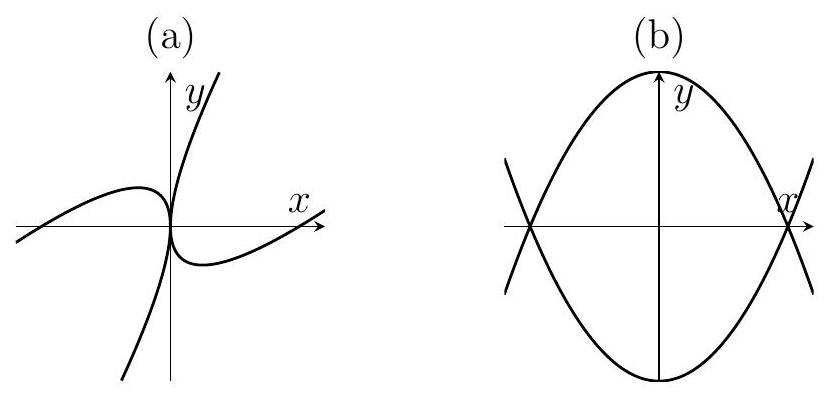
\includegraphics[max width=\textwidth, center]{2024_03_31_3a16842be9d1f70d52efg-11(2)}

(c)

\begin{center}
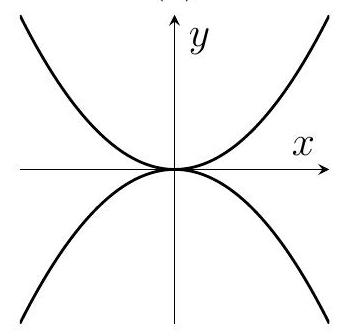
\includegraphics[max width=\textwidth]{2024_03_31_3a16842be9d1f70d52efg-11(3)}
\end{center}

(d)

\begin{center}
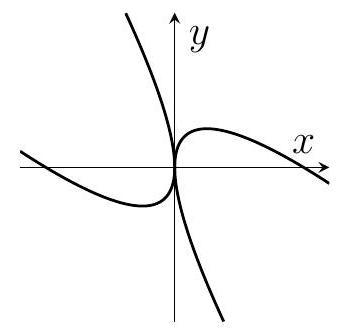
\includegraphics[max width=\textwidth]{2024_03_31_3a16842be9d1f70d52efg-11}
\end{center}

(e)

\begin{center}
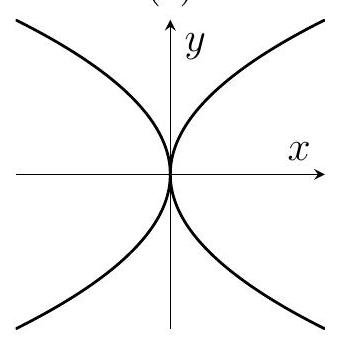
\includegraphics[max width=\textwidth]{2024_03_31_3a16842be9d1f70d52efg-11(1)}
\end{center}

End of last question


\end{document}